%
% sec-3-design.tex
%
% Embedded languages, stratified types, richly typed terms, representing
% programs. The Accelerate language.
%
% Accelerate CUDA backend. Code generation. Executing computations. Garbage
% collection. Caching.
%

% Need a better title
\chapter{Basics}  % Design of an embedded language
\epigraph{You see a wile, you thwart. Am I right?}%
{\textsc{---terry pratchett and neil gaiman}\\\textit{Good Omens}}


\section{Data Parallelism}
\label{sec:data_parallelism}

The major processor manufacturers and architectures have long since run out of
room with most of the traditional approaches to boosting CPU performance.
Instead of driving clock speed and straight-line instruction throughput,
including multiple cores on a single chip has become the dominant mechanism for
scaling processor performance. Despite this trend being apparent for a number of
years, programming parallel computers remains an extremely challenging task ---
even for expert computer programmers, let alone for scientists in other
disciplines.

One programming model that has shown to make good use of parallel hardware is
\indexe{data parallelism}.
% The idea is that the application of an operation over
% a collection of data, such as an array, can often be performed in parallel.
Data parallelism focuses on distributing the data over the available processors,
and for each processor to perform the \emph{same} task on the \emph{different}
pieces of distributed data. To the programmer, data parallelism exposes a single
logical thread of execution that is fairly easy to understand and reason about.
In addition to its simplicity, the data parallel approach to programming
parallel computers has several advantages:
%
\begin{enumerate}
\item The model is independent of the number of processors, so scales to any
    number of processors by decomposing data into the appropriate number of
    chunks.

\item All synchronisation is implicit, so the programming model is safe from
    race conditions, eliminating a major source of errors in parallel programs.

\item As memory bandwidth is often a limiting factor in modern computers, the
    emphasis on data layout can assist with both data flow as well as
    parallelisation.
\end{enumerate}
%
In the world of massively parallel computing with strong locality requirements,
data parallelism is the well established, demonstrably successful brand leader.
Examples of data parallel programming environments include High Performance
Fortran (HPF)~\cite{HPF:1997}, the collective operations of the Message Passing
Interface (MPI)~\cite{MPI:2012}, Google's Map/Reduce
framework~\cite{Dean:2008fi}, and NVIDIA's CUDA API for graphics
processors~\cite{NVIDIA:2012wf}.


\section{GPU computing} % {GPGPU programming is data parallel programming}
\label{sec:gpu_computing}

General-purpose computing on graphics processing units
(\indext{GPGPU}\index{GPGPU|see {general-purpose computing on graphics
processing units}}) is the utilisation of a graphics processing unit (\GPU),
which typically handles the computations for computer graphics, to perform
computations in applications typically handled by the central processing unit
(CPU). Since general purpose CPUs are designed to optimise the performance of a
single thread of execution, much of the processor's resources (die area and
power) to non-computational tasks such as caching and branch prediction.
Conversely, the highly parallel nature of graphics processing (rasterisation)
means the GPU architecture instead uses these resources to be able to execute
many tasks in parallel, improving the computational throughput for parallel
workloads at the expense of decreased single threaded performance. This
difference in architectures between the CPU and GPU is illustrated in
Figure~\ref{fig:cpu_gpu_block_diagram}.

\begin{figure}[tbp]
    \centering
    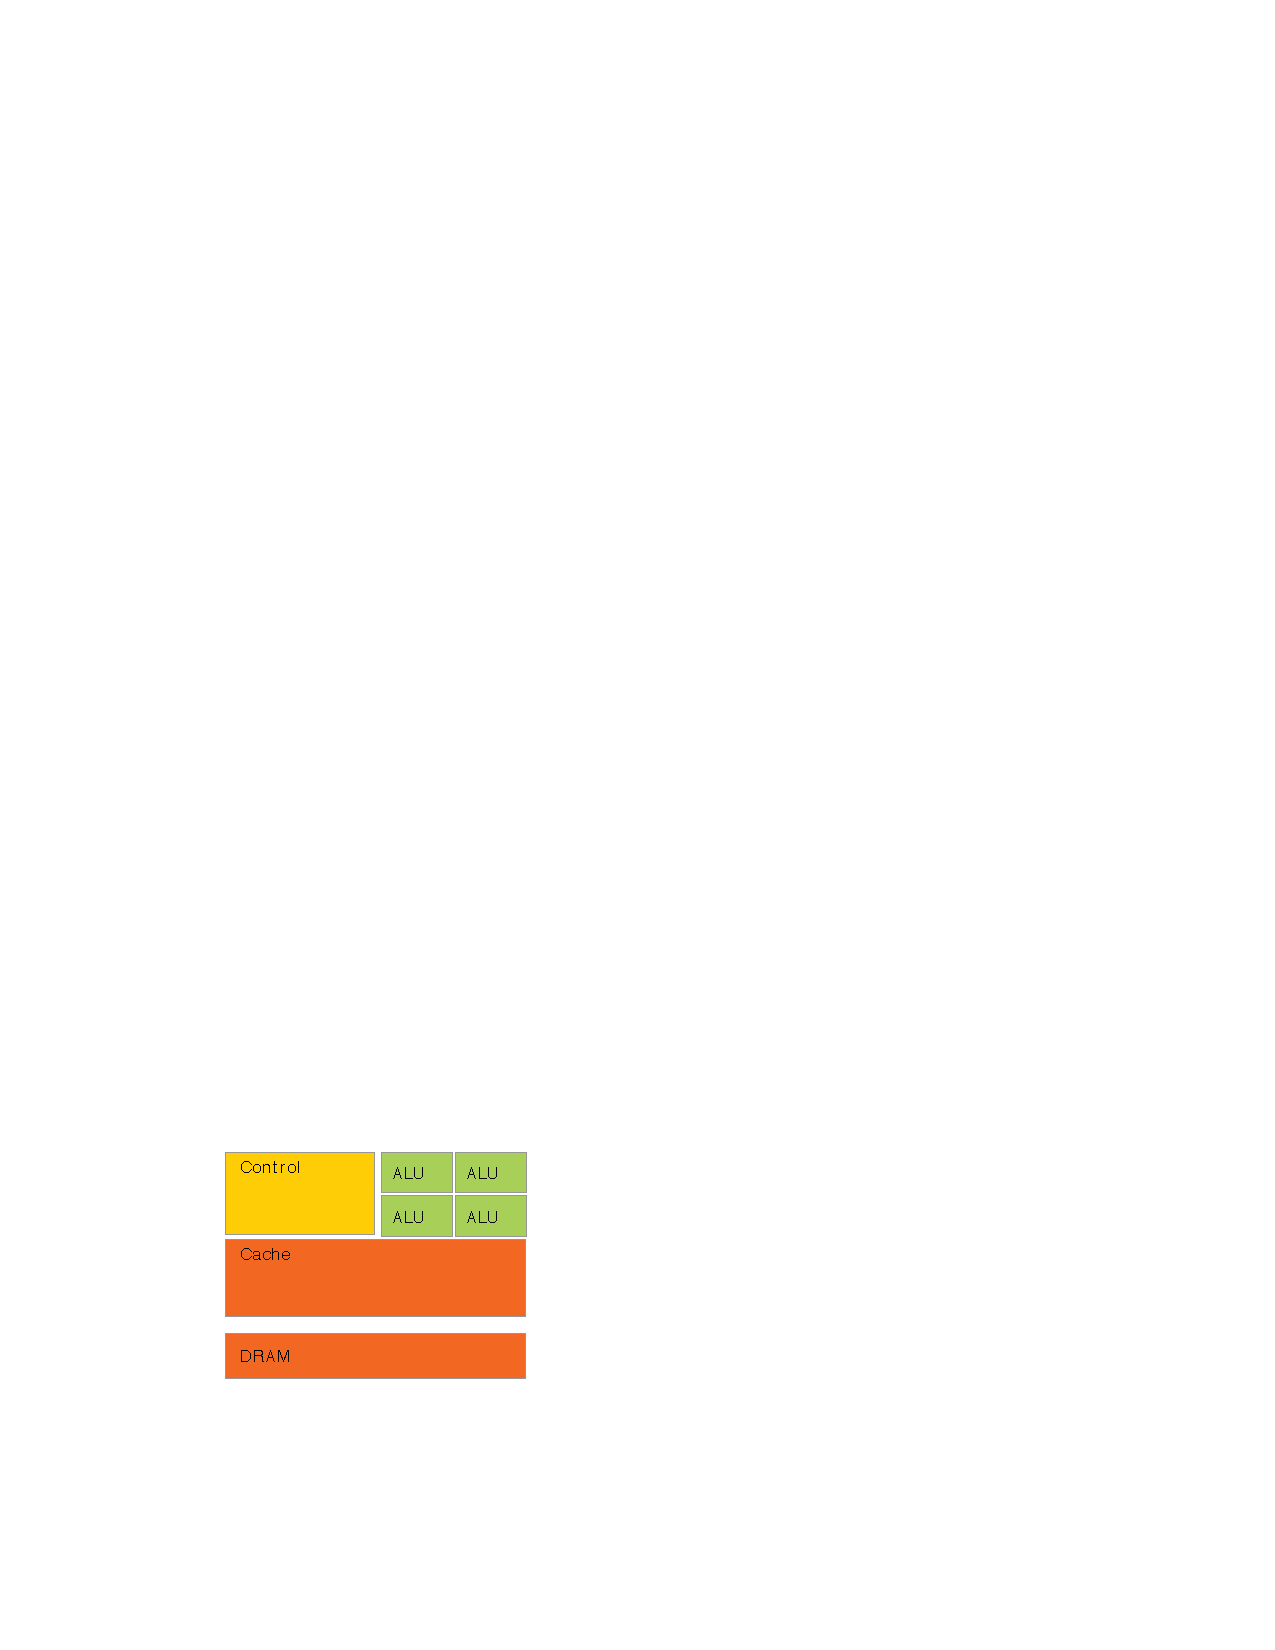
\includegraphics[width=0.4\textwidth]{images/sec-3/block_cpu}
    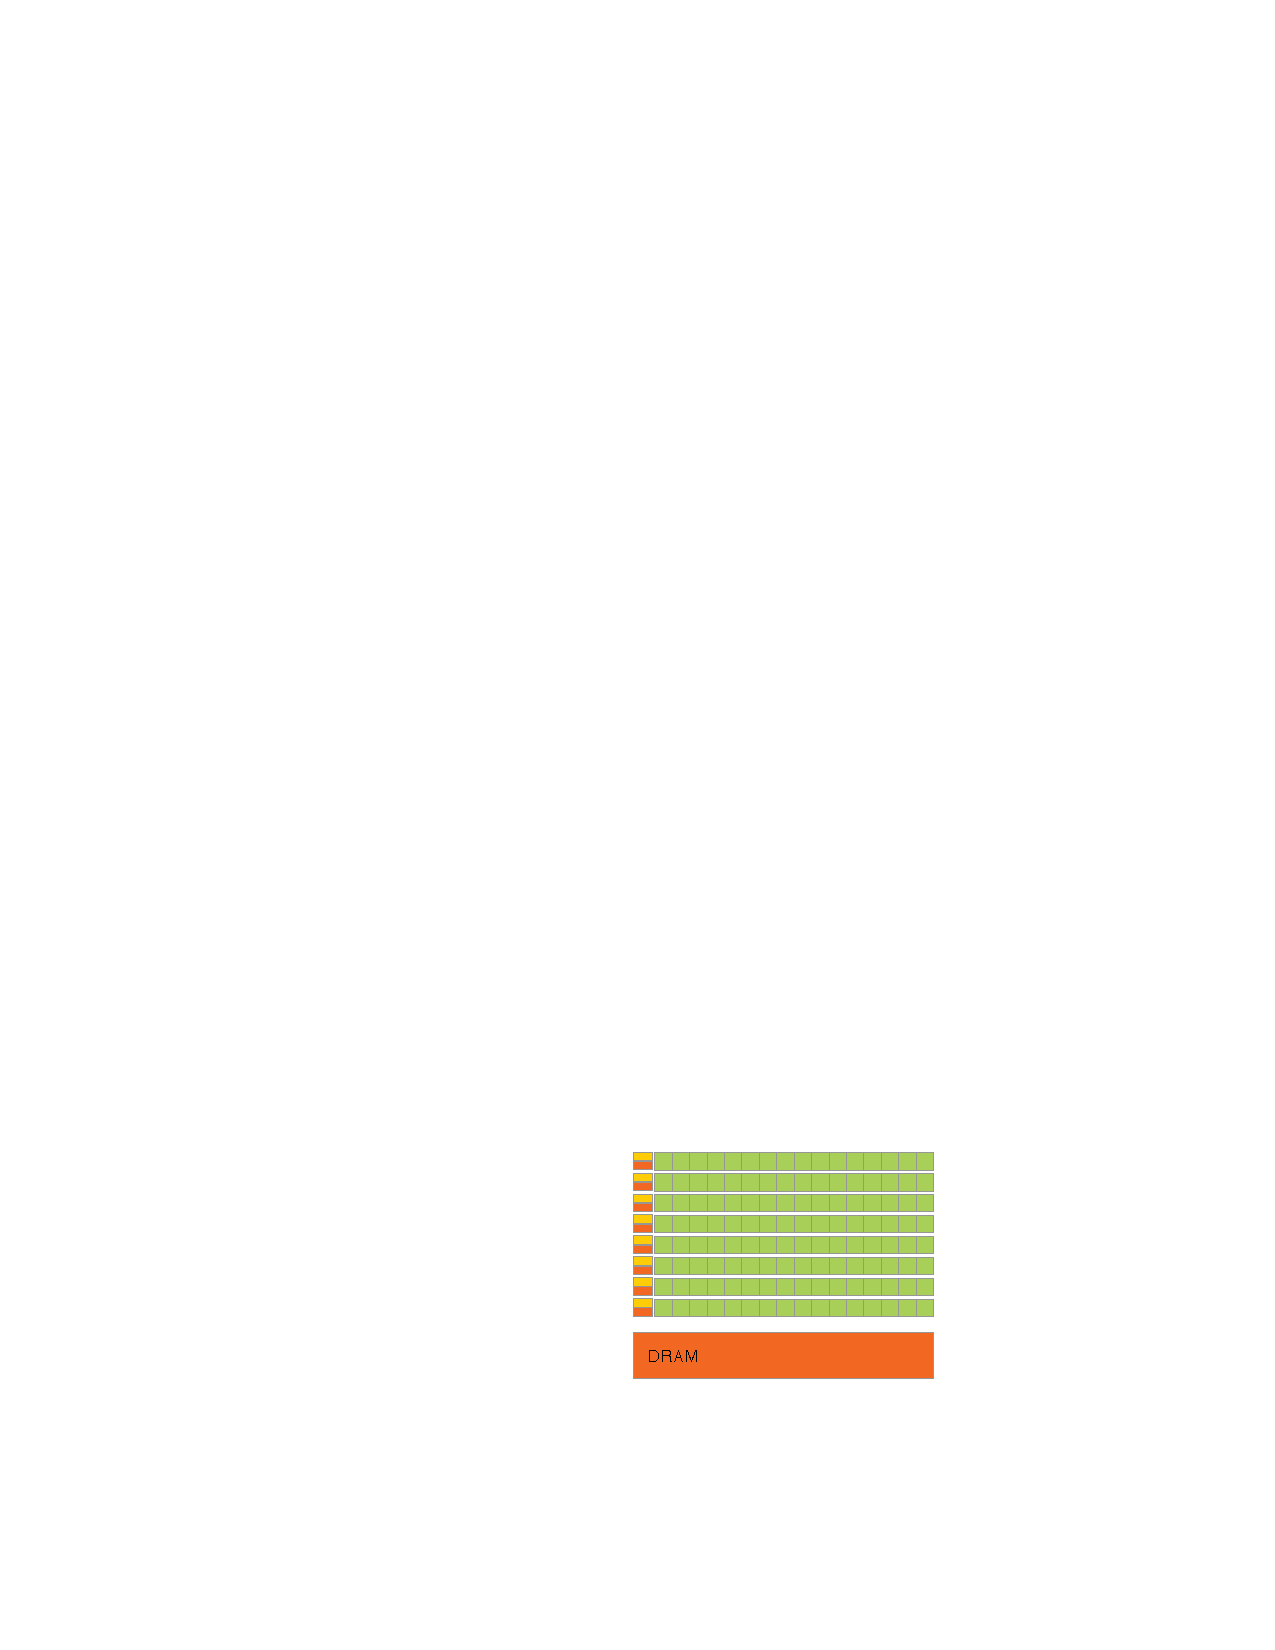
\includegraphics[width=0.4\textwidth]{images/sec-3/block_gpu}
    \caption[The GPU devotes more transistors to data processing]{Block diagram
    comparing the relative use of transistors in a CPU (left) compared to a GPU
    (right). The GPU is specialised for highly parallel, compute intensive
    workloads, and so is designed such that the majority of its transistors are
    devoted to data processing, rather than data caching and control flow.
    Images from~\cite{NVIDIA:2012wf}.}
    \label{fig:cpu_gpu_block_diagram}
\end{figure}

More specifically, the GPU is especially well suited to expressing problems that
can be expressed as data parallel computations, where the same program is
executed by many processors on many different data elements in parallel
(\S\ref{sec:data_parallelism}). Because the same program is executed by many
processors, there is no need for sophisticated control flow, and because it is
executed on many data elements, memory access latency can be hidden with
calculations rather than by big caches. Many applications that process large
data sets can use the data parallel programming model to speed up calculations,
and these applications can be coded to execute on the GPU.


\subsection{CUDA}
\label{sec:cuda}

\CUDA is the parallel computing platform and programming model created by
NVIDIA, which gives programmers direct access to the memory and parallel
computation units of their GPUs. Using CUDA, the massively parallel multicore
architecture of the GPU becomes accessible for general purpose computing, not
just graphics.

CUDA extends the C programming language by allowing the C programmer to define
functions, called \emph{kernels}\index{GPU!kernel}, that, when called, are
executed $n$ times in $n$ data parallel threads on the available processing
elements, rather than only once like regular C functions. These functions are
executed by threads arranged in a multidimensional structure of \emph{thread
blocks}\index{GPU!thread block}. Threads within a block can cooperate by sharing
data through some \emph{shared memory}\index{GPU!shared memory} and by
synchronising their execution to coordinate memory access. More precisely, the
programmer can specify synchronisation points in the kernel by calling
@__syncthreads()@\index{GPU!\code{__syncthreads()}}, which acts as a barrier at
which all threads in the block must wait before any is allowed to proceed. Each
thread block executes independently of each other, so a GPU with a higher number
of CUDA cores --- or \emph{streaming multiprocessors}\index{GPU!streaming
multiprocessor} (SM) --- will execute the program in less time than a GPU with
fewer multiprocessors.

\begin{lstlisting}[style=cuda
    ,float
    ,label=lst:cuda_vecadd
    ,caption={[CUDA kernel for pair wise addition of two vectors]A CUDA kernel
        that illustrates pair wise addition of two vectors. The
        \code{__global__} keyword marks a function as a kernel that should be
        executed on the GPU in data parallel. The execution configuration syntax
        \code{<<<...>>>} specifies the number of threads that will each execute
        the function in data parallel.}]
// Kernel definition
__global__ void VecAdd(float *A, float *B, float *C, int N)
{
    int i = blockIdx.x * blockDim.x + threadIdx.x;

    if (i < N) {
        C[i]  = A[i] + B[i];
    }
}

int main()
{
    ...
    // Kernel invocation with N threads
    int threadsPerBlock = 128;
    int numBlocks       = (N + threadsPerBlock - 1) / threadsPerBlock;
    VecAdd<<<numBlocks, threadsPerBlock>>>(A, B, C, N);
    ...
}
\end{lstlisting}

At an example, Listing~\ref{lst:cuda_vecadd} illustrates the pair wise addition
of two vectors $A$ and $B$ of size $N$ each, and stores the result in a vector
$C$. The kernel is defined with the @__global__@ declaration specifier. The
number of CUDA thread blocks and the number of threads in each block that
execute the kernel, at this invocation, is specified in the @<<<...>>>@ syntax.
Moreover, Listing~\ref{lst:cuda_vecadd} demonstrates that the GPU programming
model as exposed by CUDA is a data parallel programming model --- $N$ threads
execute $N$ individual instances of the kernel function @VecAdd@, and each
thread operates on a single element of each input array to create a single value
in the result.


\section{Embedded domain-specific languages}
\label{sec:EDSLs}

A \indexe{domain-specific language} (DSL) is a computer language specialised to
a specific problem domain. The DOT language~\cite{Graphviz:1998ui,Ellson:2001wf}
is an example of a DSL for describing graphs. This is in contrast to a general
purpose language such as Haskell~\cite{Haskell:1998}, which is broadly
applicable across domains but may lack specialised features for a particular
domain. A domain specific language is created to solve problems in a particular
domain, and is not intended to solve problems outside it (although this may be
technically possible). Restricting the problem domain the language is intended
to solve may allow for more optimisations during compilation, or increased
expressivity when representing problems or defining solutions in that domain.

An \emph{embedded} (or \emph{internal}) \emph{domain-specific
language}\index{domain-specific language!embedded} (EDSL) is a domain-specific
language that is designed to be used from within another host
language~\cite{Hudak:1996}. The embedded language is implemented as a library,
so is able to reuse the syntax and features of the general purpose host language
compiler, including compilation phases such as lexing, parsing, and semantic
analyses such as type checking, while adding domain specific elements such as
data types, or domain specific optimisations and code generation.

There are two major degrees in which an embedded language can be implemented:

\subsection{Shallow embedding}

In a shallow embedding, operations in the embedded language translate directly
into operations in the target language. A shallow embedding captures the
semantics of the data of the domain in a data type, and provides a \emph{fixed}
interpretation of that data. Thus, it is easy to add new constructs to the
language --- so long as they can be interpreted in the semantic domain --- and
the embedded language can reuse features of the host language, such as variable
binding.


\subsection{Deep embedding}

A deep embedding captures the semantics of the embedding by reflecting the
operations of the object language into a data structure. This data structure ---
an \indexe{abstract syntax tree} (AST) --- then permits transformations, such as
optimisations, before being translated into the target language. Deeply embedded
languages therefore enable a \emph{variable} interpretation of operations in the
domain, so it is easy to add new interpretations of the embedding, for example,
compiling to a different target language. However, adding new language
constructs requires extending the AST data type, and the implementation must
deal explicitly with binding of variables. Sharing and recursion are common
problems when implementing deeply embedded languages.

As the deeply embedded language runs inside of the host language, reflecting
operations into an AST, an interpreter for the embedded language must be
embedded within the host application.
% This interpreter may execute instructions in the internal language directly,
% or it may generate code that is compiled into machine language instructions to
% be executed.
As the interpreter executes code for the embedded language at program runtime,
code in the embedded language may either be written by the user or generated
dynamically by the application. If the target language is different to that of
the host language, this entails the interpreter generating, compiling, and
executing code for the target language at program runtime.


\section{The Accelerate EDSL}

The current generation of graphical processing units (GPUs) are massively
multicore processors (\S\ref{sec:gpu_computing}). They are optimised for
workloads with a large degree of data parallelism (\S\ref{sec:data_parallelism})
and good performance depends on highly idiomatic programs with low SIMD
divergence and regular memory-access patterns. Hence, the development of
applications that use the graphics processors for general purpose computations
(\S\ref{sec:gpu_computing}) is work intensive and requires a substantial degree
of expert knowledge.

Accelerate is our approach to reducing the complexity of GPU programming: a
high-level, deeply embedded domain-specific language (\S\ref{sec:EDSLs}) of
array computations that captures appropriate GPGPU idioms in the form of
parameterised, \indexe{rank-polymorphic}~\cite{Keller:2010er}, collective
operations on arrays~\cite{Chakravarty:2011fr}. Our choice of operations was
informed by the \emph{scan-vector model}~\cite{Chatterjee:1990vj}, which is
suitable for a wide range of algorithms, and demonstrated that these operations
can be efficiently implemented on modern GPUs~\cite{Sengupta:2007tc}.

We regard Accelerate's collective array operations as algorithmic
skeletons~(\S\ref{sec:code_generation}) that capture appropriate GPU programming
idioms. The dynamic code generator instantiates CUDA implementations of these
skeletons~(\S\ref{sec:parallel_algorithms_in_cuda}) to implement embedded array
programs~(\S\ref{sec:instantiating_skeletons}). Dynamic code generation exploits
runtime information of the target hardware to optimise GPU code, and enables
on-the-fly generation of embedded array programs by the host
program~(\S\ref{sec:dynamic_compilation}). The evaluator minimises the overhead
of dynamic code generation by caching binaries of previously compiled skeleton
instantiations and by parallelising code generation, data
transfer~(\S\ref{sec:memory_management}), and GPU kernel loading, configuration,
and execution~(\S\ref{sec:executing_programs}).

To achieve performance competitive with hand-written
CUDA~\cite{McDonell:2013wi}, we implement two primary optimisation techniques:
sharing recovery~(\S\ref{sec:sharing_recovery}) tackles code explosion due to
the embedding in Haskell, while array
fusion~(\S\ref{sec:implementing_array_fusion}) eliminates superfluous
intermediate structures, which often arise due to the high-level nature of the
language. Both of these techniques are well known from other contexts, but they
present unique challenges for an embedded language compiled for execution on a
GPU.

\begin{figure}
    \centering
    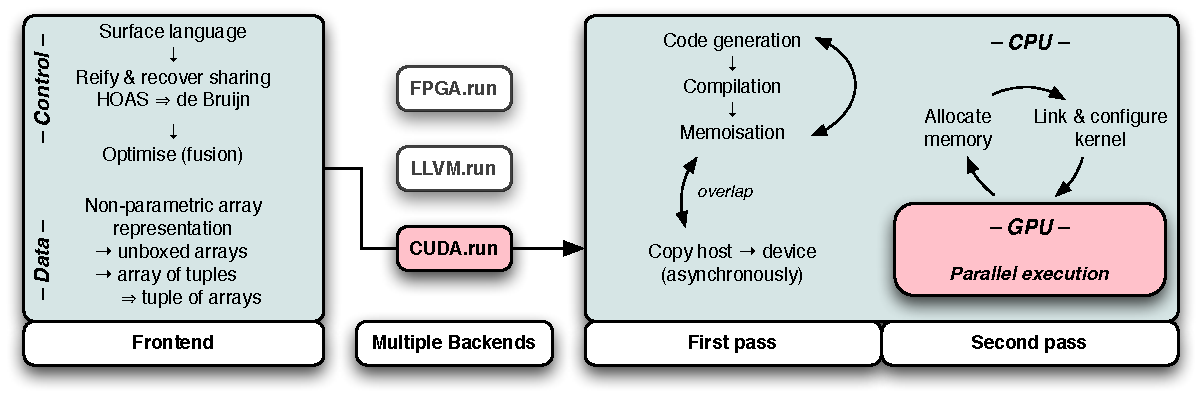
\includegraphics[width=\textwidth]{images/sec-3/outline-s}
    \caption[The overall structure of Accelerate]{The overall structure of
    Accelerate. It comprises a frontend and supports multiple backends that can
    target a variety of architectures.}
    \label{fig:outline}
\end{figure}

Figure~\ref{fig:outline} summarises the overall structure of Accelerate. It
comprises a frontend and support for multiple backends that can target a variety
of architectures. Here, we are only concerned with the CUDA generating GPU
backend, but the approach is amenable to targeting multicore CPU backends
exploiting SIMD instructions, backends for OpenCL, and for reconfigurable
hardware such as FPGAs. In the following, we briefly introduce some features of
the design and use of Accelerate.


\subsection{Computing a vector dot product}
\label{sec:computing_dotp}

Consider computing the dot product of two vectors, using standard Haskell lists:
%
\begin{lstlisting}[style=haskell]
dotp_list :: [Float] -> [Float] -> Float
dotp_list xs ys = foldl (+) 0 (zipWith (*) xs ys)
\end{lstlisting}
%
The two input vectors @xs@ and @ys@ are pointwise multiplied, and the resulting
list of products is summed, yielding the scalar result.

Using Accelerate, we implement this computation on arrays as follows:
%
\begin{lstlisting}[style=haskell]
dotp :: Vector Float -> Vector Float -> Acc (Scalar Float)                         -- (1)
dotp xs ys
  = let xs' = use xs                                                               -- (2)
        ys' = use ys
    in
    fold (+) 0 (zipWith (*) xs' ys')                                               -- (3)
\end{lstlisting}
%
Here, @fold@ and @zipWith@ are taken from the Accelerate library
@Data.Array.Accelerate@, rather than from the standard Haskell library
@Data.List@. The Accelerate code differs from the list version in three
respects:
%
\begin{enumerate}
    \item The result is an Accelerate computation, indicated by the type @Acc@.
    \item We lift the two plain vectors @xs@ and @ys@ into @Acc@ terms with @use@.
    \item We use @fold@ instead of @foldl@.
\end{enumerate}
%
The first two points are artefacts of lifting the computation into an embedded
language, effectively delaying the computation. Concerning the final point, the
list traversal function @foldl@ guarantees a left-to-right traversal of the
elements, whereas @fold@ leaves the order in which the elements are combined
unspecified. This requires that the binary operator supplied to @fold@ is
associative and commutative,\footnote{Although floating-point arithmetic is not
strictly associative, it is common to accept the resulting error in parallel
applications.} but allows for an implementation using a parallel tree
reduction~\cite{Chatterjee:1990vj,Sengupta:2007tc}.


\subsection{Arrays, shapes, and indices}
\label{sec:arrays_shapes_and_indices}

Parallelism in Accelerate takes the form of collective operations on arrays of
type @Array sh e@, where @sh@ is the \emph{shape} and @e@ the \emph{element
type} of the array. Following the approach taken in Repa~\cite{Keller:2010er},
we represent both the shapes and indices of an array using an inductive notation
of tuples as heterogeneous \emph{snoc} lists to enable rank-polymorphic
definitions of array functions.

As shown in Listing~\ref{lst:shapes_and_indices}, on both the type and value
level, the constructor @Z@ is used to represent the shape of a rank-0 array, and
the infix operator @(:.)@ to increase the rank by adding a new (innermost)
dimension to the right of the shape. Thus, a rank-3 index with components @x@,
@y@, and @z@, is written @(Z:.z:.y:.x)@ and has type @(Z:.Int:.Int:.Int)@, where
the component @x@ is innermost and varies most rapidly, while the component @z@
varies least rapidly.

\begin{lstlisting}[style=haskell
    ,float
    ,label=lst:shapes_and_indices
    ,caption={Types of array shapes and indices}]
data Z            = Z                   -- rank zero
data tail :. head = tail :. head        -- increase rank by one

type DIM0 = Z
type DIM1 = DIM0 :. Int
type DIM2 = DIM1 :. Int
type DIM3 = DIM2 :. Int
  -- $\langle$ and so on $\rangle$

type Array DIM0 e = Scalar e
type Array DIM1 e = Vector e
\end{lstlisting}

Overall, an array of type @Array (Z:.Int:.Int) Float@ is a rank-2 array of
single precision floating-point numbers. Listing~\ref{lst:shapes_and_indices}
also defines synonyms for common array types: a singleton array of shape @DIM0@
represent a single scalar value, while an array of shape @DIM1@ represents a
vector, and so on. While it may appear that the explicit mentioning of @Int@ in
each dimension is redundant, we require indices over types other than @Int@ for
rank polymorphic functions, such as replicating an array into one or more
additional dimensions or slicing a lower-dimensional subarray out of a larger
array~\cite{Keller:2010er}.


\subsection{Arrays on the host and device}
\label{sec:arrays_on_the_host_and_device}

Accelerate is an \emph{embedded language} (\S\ref{sec:EDSLs}) that distinguishes
between vanilla Haskell arrays and arrays in the embedded language, as well as
computations on both flavours of arrays. Embedded array computations are
identified by types formed from the type constructor @Acc@, and must be
explicitly executed before taking effect. The following function embeds a
Haskell array into an embedded array computation:
%
\begin{lstlisting}[style=haskell]
  use :: (Shape sh, Elt e)
      => Array sh e -> Acc (Array sh e)
\end{lstlisting}
%
In the context of GPU programming, GPUs typically have their own
high-performance memory which is separate from the host CPU's main memory, and
data must be explicitly transferred to the GPU's memory before it can be used.
The distinction between regular arrays of type @Array sh e@ and arrays of the
embedded language @Acc (Array sh e)@ has the added benefit of differentiating
between arrays allocated in host memory and arrays allocated in GPU device
memory. Thus, @use@ also implies a host-to-device data transfer. See
section~\ref{sec:memory_management} for more information on how device memory is
managed. Similarly, expressions in @Acc@ are computations that are executed on
the device, whereas regular Haskell code runs on the host.


\subsection{Array computations versus scalar expressions}
\label{sec:array_computations_vs_scalar_expressions}

The signatures of the two operations @zipWith@ and @fold@, using in the
definition of @dotp@, are shown in Listing~\ref{lst:acc_operations}. These
operations follow the signatures of the corresponding list functions, but with
arrays wrapped in @Acc@. In addition to @Acc@, which marks embedded array
computations, we also have @Exp@, which marks \emph{embedded scalar}
computations: a term of type @Exp Int@ represents an embedded expression
yielding a value of type @Int@, and similarly @Exp Float -> Exp (Float,Float)@
characterises an embedded scalar function that takes an argument of type @Float@
and yields a pair of @Float@s as the result. As with computations embedded in
@Acc@, computations in @Exp@ are executed on the device.

\begin{lstlisting}[style=haskell,
    numbers=none,
    float=t,
    label={lst:acc_operations},
    caption={[Core Accelerate array operations] Summary of Accelerate's core
        collective array operations, omitting \code{Shape} and \code{Elt} class
        constraints for brevity. In addition, there are other flavours of folds
        and scans as well as segmented versions of these.}]
-- Embed an array
use :: Array sh e -> Acc (Array sh e)

-- Create a singleton array
unit :: Exp e -> Acc (Scalar e)

-- Impose a new shape on an array
reshape :: Exp sh -> Acc (Array sh' e) -> Acc (Array sh e)

-- Create an array from an index mapping
generate :: Exp sh -> (Exp sh -> Exp a) -> Acc (Array sh a)

-- Extend an array across new dimensions; remove existing dimensions
replicate :: Slice slix
          => Exp slix -> Acc (Array (SliceShape slix) e) -> Acc (Array (FullShape slix) e)
slice     :: Slice slix
          => Acc (Array (FullShape  slix) e) -> Exp slix -> Acc (Array (SliceShape slix) e)

-- May a function over an array; over a pair of arrays
map     :: (Exp a -> Exp b) -> Acc (Array sh a) -> Acc (Array sh b)
zipWith :: (Exp a -> Exp b -> Exp c)
        -> Acc (Array sh a) -> Acc (Array sh b) -> Acc (Array sh c)

-- Tree reduction along the innermost dimension
fold :: (Exp a -> Exp a -> Exp a) -> Exp a -> Acc (Array (sh:.Int) a) -> Acc (Array sh a)

-- Left-to-right or right-to-left vector pre-scan
scan{l,r} :: (Exp a -> Exp a -> Exp a) -> Exp a -> Acc (Vector a) -> Acc (Vector a)

-- Rearrange elements based on backwards, forwards index mapping
backpermute :: Exp sh' -> (Exp sh' -> Exp sh) -> Acc (Array sh a) -> Acc (Array sh' e)
permute     :: (Exp a -> Exp a -> Exp a) -> Acc (Array sh' a)
            -> (Exp sh -> Exp sh') -> Acc (Array sh a) -> Acc (Array sh' a)

-- Map a function with local neighbourhood context
stencil :: Stencil sh a stencil
        => (stencil -> Exp b) -> Boundary a -> Acc (Array sh a) -> Acc (Array sh b)
\end{lstlisting}

Accelerate distinguishes the types of collective and scalar computations to
achieve a stratified language. Collective operations in @Acc@ comprise many
scalar computations in @Exp@ that are executed in parallel. However, scalar
computations \emph{can not} contain collective operations. This stratification
excludes \emph{nested, irregular} data parallelism statically --- instead,
Accelerate is limited to \emph{flat data-parallelism} involving only regular,
multi-dimensional arrays.

Compared to regular Haskell, @Exp@ computations are rather limited in order to
meet the restrictions of what can be efficiently executed on GPUs. In
particular, we do not support recursion, and provide only a limited form of
explicit iteration. Scalar expressions support Haskell's standard arithmetic
operations by overloading the standard type classes such as @Num@, @Integaral@,
as well as bitwise operations from @Bits@. Although we can not overload
functions on @Bool@ in standard Haskell, we support equality and comparison
operators as well as logical connectives using the operators @(==*)@, @(/=*)@,
@(<*)@, \lstinline[style=inline,literate=]{(<=*)},      % don't turn into (≤*)
and so on. We also have conditional expressions in the form of @c ? (t, e)@,
which evaluates to @t@ if @c@ yields @True@, otherwise to @e@. There are also
scalar operations that take array valued arguments; namely, @arr!ix@ indexes an
array and @shape@ queries an arrays extent. The argument to these operations is
guaranteed to only be a previously let-bound variable, thus each invocation of
the scalar function will not initiate additional parallel work. Finally, we have
tupling and projection, and auxiliary functions for computing with indices.


\subsection{Computing an N-body gravitational simulation}
\label{sec:computing_nbody}

At a second example, consider simulating the Newtonian gravitational forces on a
set of massive bodies in 3D space, using a na\"ive O($n^2$) algorithm. We use
the following type synonyms to represent bodies in the simulation:
%
\begin{lstlisting}[style=haskell]
type Vec a      = (a, a, a)
type Position   = Vec Float
type Accel      = Vec Float

type Mass       = Float
type PointMass  = (Position, Mass)
\end{lstlisting}
%
@Vec@ is the type of 3-component vectors, which are used to store the $x$-, $y$,
and $z$-components of the particle's position in 3D space and velocity component
along each dimension in @Position@ and @Accel@ respectively. A @PointMass@
is represented as a tuple containing the body's @Mass@ and @Position@.

In a data-parallel setting, the natural implementation first computes the forces
between every pair of bodies, before reducing the components applied to each
body using a segmented sum. In Accelerate, we can calculate the acceleration
each body experiences as it interacts with all other bodies in the system as
follows:
%
\begin{lstlisting}[style=haskell]
calcAccels :: Exp R -> Acc (Vector PointMass) -> Acc (Vector Accel)
calcAccels epsilon bodies
  = let n       = A.size bodies
        cols    = A.replicate (lift $ Z :. n :. All) bodies                        -- (1)
        rows    = A.replicate (lift $ Z :. All :. n) bodies
    in
    A.fold (.+.) (vec 0) $ A.zipWith (accel epsilon) rows cols                     -- (2)
\end{lstlisting}
%
\begin{enumerate}
\item @replicate@ expands the vector of @n@ bodies into an @n@$\times$@n@
    matrix, where we replicate @All@ elements of the source array such that
    every element down the columns or along the rows of the matrix are
    identical, respectively. The operation @lift@ is used to push the shape
    constructors into the expression; that is, in this instance we have
    @lift :: (Z :. Exp Int :. All) -> Exp (Z :. Int :. All)@.

\item @zipWith@ calculates the interaction between each pair of particles by
    element wise combining the @n@$\times$@n@ matrices. @fold@ reduces the
    result along the innermost dimension only, yielding a vector containing the
    sum of interactions for each particle between all others. The auxiliary
    function performs @(.+.)@ is component-wise addition of the 3-vector.
\end{enumerate}

This is an example of using the rank polymorphic operations of Accelerate. The
function @fold@ requires an argument array of at least rank-1 (such as a
matrix), and the result is computed by reducing the array along the innermost
dimension, reducing the rank of the array by one (in this case a vector). The
functions @replicate@ and @slice@ are rank polymorphic as well, but require more
complex shape constraints that we characterise with the type family @FullShape@
and @SliceShape@ that statically track changing array dimensions. For details on
the various forms of shape polymorphism, see~\cite{Keller:2010er}. Overall, as
shown in Listing~\ref{lst:acc_operations}, the collective operations of
Accelerate are a multi-dimensional variant of those underlying the scan-vector
model~\cite{Chatterjee:1990vj,Sengupta:2007tc}.


\subsubsection{Computing gravitational potential}

We briefly explain how to compute the gravitational potential between a pair of
bodies. Given $n$ bodies with position $\mathbf{x}_i$ and velocity
$\mathbf{v}_i$ for $i \in [1,n]$ (bold face indicates a 3-component vector), the
force $\mathbf{f}_{ij}$ on a body $i$ is caused by its gravitational attraction
to body $j$:
%
\begin{equation*}
    \mathbf{f}_{ij}
      = G \frac{m_i m_j}{\|\mathbf{r}_{ij}\|^2}
        \cdot
        \frac{\mathbf{r}_{ij}}{\|\mathbf{r}_{ij}\|}
\end{equation*}
%
where $m_i$ and $m_j$ are the masses of the bodies, $\mathbf{r}_{ij} =
\mathbf{x}_j - \mathbf{x}_i$ is the vector from body $i$ to body $j$, and $G$ is
the gravitational constant. The factor on the left represents the
\emph{magnitude} of the acceleration, and is proportional to the product of the
masses and diminishes as the square of the separation of the masses. The right
factor is the \emph{direction} of the force, and is the unit vector from $i$ in
the direction of $j$.

The total force $\mathbf{F}_i$ on a body $i$ due to its interactions with the
other bodies is thus:
%
\begin{equation*}
    \mathbf{F}_i
      = \sum_{\substack{1 \le j \le n\\j \ne i}} \mathbf{f}_{ij}
      = G m_i \cdot \sum_{\substack{1 \le j \le n\\j \ne i}}
            \frac{m_j \mathbf{r}_{ij}}{\|\mathbf{r}_{ij}\|^3}
\end{equation*}
%
Note that as the bodies approach each other, the force between them grows
without bound, which is undesirable for numerical simulations. In astrophysical
simulation, collisions between bodies are generally precluded, which is
reasonable if the bodies represent galaxies that may pass through each other. A
\emph{softening factor} $\epsilon^2 > 0$ is added, which models the interaction
of two Plummer point masses~\cite{Aarseth:2003uz,Dyer:1993bk}. In effect,
softening limits the magnitude of forces between bodies. The denominator is
rewritten as follows:
%
\begin{equation*}
    \mathbf{F}_i \approx G m_i \cdot \sum_{1 \le j \le n}
        \frac{m_j \mathbf{r}_{ij}}
             {\left( \|\mathbf{r}_{ij}\| + \epsilon^2 \right)^{\sfrac{3}{2}}}
\end{equation*}
%
The condition $j \ne i$ is no longer needed, because $\mathbf{f}_{ii} = 0$ when
$\epsilon^2 > 0$.

Finally, the acceleration experienced by a body is $\mathbf{a}_i =
\mathbf{F}_i/m_i$, and we can now present the Accelerate routine to compute the
accelerate between two bodies.
%
%\begin{equation*}
%    \mathbf{a}_i \approx
%    G \sum_{1 \le j \le n}
%      \frac{m_j \mathbf{r}_{ij}}
%           {\left( \|\mathbf{r}_{ij}\|^2 + \epsilon^2 \right)^{\sfrac{3}{2}}}
%\end{equation*}
%
%
\begin{lstlisting}[style=haskell]
accel :: Exp R -> Exp PointMass -> Exp PointMass -> Exp Accel
accel epsilon pmi pmj = (mj * invr3) *. r
  where
    mj          = massOfPointMass pmj
    r           = positionOfPointMass pmj .-. positionOfPointMass pmi
    rsqr        = dot r r + epsilon * epsilon
    invr        = 1 / sqrt rsqr
    invr3       = invr * invr * invr
\end{lstlisting}
%
Here, a @PointMass@ is represented as a tuple containing the body's position in
3D space together with its mass, and functions @positionOfPointMass@ and
@massOfPointMass@ extract each component, respectively. The function @(.-.)@ is
component-wise subtraction applied to the 3-vector, and @(*.)@ multiplies each
component of a 3-vector by a scalar value.


\subsection{Non-parametric array representation}

In the type signature of @use@ in
section~\ref{sec:arrays_on_the_host_and_device}, the type classes @Shape@ and
@Elt@ characterise the types that may be used as array indices and array
elements respectively. We discussed the nature of array indices in
section~\ref{sec:arrays_shapes_and_indices}. The @Elt@ characterises the types
of values that can be used as array elements, and hence appear in scalar
Accelerate expressions. The supported @Elt@ are signed \& unsigned integers (8,
16, 32, and 64-bit wide), floating point numbers (single \& double precision),
as well as @Char@, @Bool@, and array indices formed from @Z@ and @(:.)@.
Furthermore, there are tuples of all of those, including nested tuples, as was
seen in the N-body example~(\S\ref{sec:computing_nbody}).

Accelerate arrays of primitive type, such as @Int@ and @Float@, are easily
represented as arrays of the corresponding integral and floating point types.
More interesting is the case of arrays of tuples, where we use a non-parametric
array representation so that arrays of tuples are represented in memory as a
tuple of arrays, one array for each primitive type in the structure. By virtue
of this representation, Accelerate is able to make optimal use of the available
memory bandwidth. See section~\ref{sec:representing_tuples} for details.

Moreover, consider the following types:
%
\begin{lstlisting}[style=haskell]
data Point = P Int Int

point :: Exp Point
sh    :: Exp (Z :. Int :. Int)
tup   :: Exp (Int, Int)
\end{lstlisting}
%
The salient feature of each expression is that it returns two integers, albeit
each wrapped in different constructors. We call this the \emph{surface} type
of a term. However, an Accelerate backend implementation should not need to know
about the surface type representation, and certainly, we should not need to
extend the backend to support user-defined types such as @Point@. The @Elt@
class tells us how to convert between the surface type of an expression that a
user programs in, into the \emph{representation} type that an implementation
stores and computes data in. We use a type
family~\cite{Chakravarty:2005dx,Schrijvers:2008ir} of nested tuples to represent
types as heterogenous snoc-lists of primitive types.
%
\begin{lstlisting}[style=haskell]
type family EltRepr a :: *
type instance EltRepr ()        = ()
type instance EltRepr Int       = ((), Int)
type instance EltRepr Float     = ((), Float)
type instance EltRepr (a, b)    = (EltRepr a, EltRepr' b)
type instance EltRepr (a, b, c) = (EltRepr (a, b), EltRepr' c)
  -- and so on\ldots
\end{lstlisting}
%
Here @EltRepr'@ is similar, except that we use a flattened representation at the
leaves in order to avoid overly nested pairs; that is, primitive types are
represented as @EltRepr' Int = Int@. Arrays of tuples have a similar mapping
into a nested tuple of arrays of primitive type.


\subsection{Richly typed terms}

\marginnote{tk: this bit is very implementation-y}
As a deeply embedded language, the operations of both the array and scalar
sub-language do not directly issue computations; instead, they build term trees
to represent embedded computations (\S\ref{sec:EDSLs}). The terms in the surface
language use \indexe{higher-order abstract syntax} (HOAS) to embed
function-valued scalar expressions as well as type class overloading to reflect
arithmetic expressions. For example, the body of the @dotp@ function
% @fold (+) 0 (zipWith (*) xs' ys')@
is translated into:\footnote{The subterms to \footcode{add} and \footcode{mul}
here are inline into the \footcode{Fold} and \code{ZipWith} terms respectively,
we only use a \footcode{where}-clause to improve readability.}
%
\begin{lstlisting}[style=haskell]
  Fold add (Const 0) (ZipWith mul xs' ys')
  where
    add = \x y -> PrimAdd (FloatingNumType (TypeFloat FloatingDict))               -- (1)
                  `PrimApp`
                  Tuple (NilTup `SnocTup` x
                                `SnocTup` y)
    mul = %$\langle$ ... as \texttt{add}, but using \texttt{PrimMul} ... $\rangle$
\end{lstlisting}
%
This is very much like the approach taken by \citet{Elliott:2004hh},
\citet{Gill:2011wy}, and \citet{Mainland:2010vj}. The difference is that in our
approach we use GADTs~\cite{Jones:2006eh} and type
families~\cite{Chakravarty:2005dx,Schrijvers:2008ir} to preserve the embedded
program's type information in the term tree (1), and use type-preserving
transformations in the front end (\S\ref{sec:manipulating_embedded_programs}).

The HOAS representation, while convenient for a human human reader, is awkward
for program transformations as it complicates looking under lambdas; i.e.
inspecting and manipulating the bodies of function abstractions. After the
frontend reifies the embedded program using HOAS, it recovers sharing
(\S\ref{sec:sharing_recovery}) while converting the HOAS representation into a
\emph{nameless} representation using \emph{typed de Bruijn indices} in the style
of~\citet{Altenkirch:2003kz}. The type preserving conversion from HOAS to a
nameless de Bruijn representation using GADTs~\cite{Chakravarty:2009uo} was
simultaneously discovered by~\citet{Atkey:2009dj}.

Overall, the nameless form of @dotp@ is:
%
\begin{lstlisting}[style=haskell]
  Fold add (Const 0) (ZipWith mul xs' ys')
  where
    add = Lam (Lam (Body (
        PrimAdd (FloatingNumType (TypeFloat FloatingDict))
                `PrimApp`
                Tuple (NilTup `SnocTup` (Var (SuccIdx ZeroIdx))
                              `SnocTup` (Var ZeroIdx)))))
    mul = %$\langle$ ... as \texttt{add}, but using \texttt{PrimMul} ... $\rangle$
\end{lstlisting}
%
The @Lam@ constructor introduces nameless abstractions and @Var@ wraps a de
Bruijn index. At this point, the program is further optimised by the frontend,
for example by applying the fusion transformation~(\S\ref{sec:array_fusion}).

Finally, we represent the environment as a heterogenous snoc-list, encoded on
the type level as nested pairs and building this list on the value level with
the two constructors:
%
\begin{lstlisting}[style=haskell]
data Val env where
  Empty :: Val ()
  Push  :: Val env -> t -> Val (env, t)
\end{lstlisting}
%
A nameless de Bruijn index projects out a specific type from the environment:
%
\begin{lstlisting}[style=haskell]
data Idx env t where                            -- an index is either\ldots
  ZeroIdx ::              Idx (env, t) t        -- \ldots at the top of the stack, or\ldots
  SuccIdx :: Idx env t -> Idx (env, s) t        -- \ldots under some junk
\end{lstlisting}
%
Indices have type @Idx env t@, where the type @env@ keeps track of what
variables are in scope using the same encoding of nested tuples used by the
environment, while @t@ represents the type of a distinguished element in this
list. At the value level, @Idx@ encodes the index of that element in the list.

As terms are pushed into the environment, the type of the new term becomes
wrapped in the type of the environment; i.e. @t@ is existentially quantified in
@Push@. Our de Bruijn indices recover the wrapped type of individual elements by
projecting the index through the environment:
%
\begin{lstlisting}[style=haskell]
prj :: Idx env t -> Val env -> t
prj ZeroIdx       (Push _   v) = v
prj (SuccIdx idx) (Push val _) = prj idx val
prj _             _            = error "inconsistent valuation"
\end{lstlisting}

\marginnote{tk: use Let/Alet constructor as further example?}
Overall, this is an example of using nested datatypes and polymorphic recursion
to precisely enforce constraints and invariants in the type of a term; in this
case the type and scope of bound terms. Since an embedded Accelerate program is
constructed and evaluated at program \emph{runtime}, encoding properties in the
type means that these invariants are checked at \emph{compile} time, reducing
the number of possible runtime errors in type-correct programs.


\section{Related work}

The development of general-purpose applications that run on the GPU is highly
work intensive, and has been estimated to require at least $10\times$ as much
effort as developing an efficient single-threaded
application~\cite{Sweeney:2009ua}. Several researchers have proposed to
ameliorate the status quo by either using a high-level library to compose GPU
code or by compiling a subset of a high-level language to low-level GPU code.
% This section explores some of these approaches.


%% Haskell-based approaches

Vertigo~\cite{Elliott:2004hh} is an embedded language in Haskell for GPGPU
programming. Vertigo is a statically compiled graphics language targeting the
DirectX 8.1 shader model, and does not offer higher-order combinators such as
@map@ and @fold@.

Obsidian~\cite{Svensson:2008a} and Nikola~\cite{Mainland:2010vj} are also
Haskell EDSLs for GPGPU programming, and are in aim and spirit the embeddings
closest to Accelerate. Both Nikola and Obsidian produce CUDA code as we do,
however while we use algorithmic skeletons (\S\ref{sec:code_generation}), Nikola
explicitly schedules loops, and Obsidian is a lower level language where more
details of the GPU hardware are exposed to the programmer. Moreover, the
Accelerate language is more expressive, supporting generative functions such as
@replicate@, and Accelerate computations can span multiple GPU kernels, whereas
both Nikola and Obsidian can only express array computations that can be
implemented in a single GPU kernel. Algorithms spanning multiple kernels need to
be explicitly scheduled by the application programmer and incur additional
host-device data transfer overhead, which can be rather significant.

% \marginnote{tk: to related work for fusion?}
% Recent versions of Obsidian~\cite{Claessen:2012hl} implement
% Repa-style~\cite{Keller:2010er} delayed \emph{pull arrays} as well as \emph{push
% arrays}. Whereas a pull array represents a general producer, a push array
% represents a general consumer. Pull arrays allow intermediate programs to be
% written in continuation passing style (CPS)\index{continuation passing style},
% which helps to compile (and fuse) append-like operations.

Paraiso~\cite{Muranushi:2012eh} is a Haskell EDSL for solving systems of
\indext{partial differential equation}s (PDEs), such as hydrodynamics equations,
and generates both CUDA code for GPUs as well as OpenMP~\cite{OpenMP:2008} code
for multicore CPUs. Accelerate supports @stencil@ operations for expressing this
type of operation, but currently lacks a backend for multicore CPUs. Paraiso
also includes an automated tuning framework to search for faster implementations
of the algorithm.

Baracuda~\cite{Larsen:2011fa} is a Haskell EDSL producing CUDA GPU kernels,
though it is intended to be used offline, with the kernels called directly from
a C++ application. It supports only @map@ and @fold@ operations.

NDP2GPU~\cite{Bergstrom:2012bi} compiles NESL~\cite{Blelloch:1995ut} code to
CUDA. Performance suffers because the implementation relies on the legacy NESL
compiler, which produces a significant number of intermediate computations.


%% C++-based approaches

Accelerator~\cite{Bond:2010bd,Tarditi:2006} is a C++ library-based approach with
less syntactic sugar for the programmer, but bindings to functional languages.
In contrast to our current work, it already targets multiple architectures,
namely GPUs, FPGAs, and multicore CPUs. However, the code generated for GPUs
uses the DirectX 9 API, which does not provide access to several modern GPU
features, negatively impacting performance and preventing some operations such
as scatted writes.

RapidMind~\cite{LinXu:2008ig}, which targets the GPU using OpenCL, and its
predecessor Sh~\cite{McCool:2004,McCool:2004un} which used pixel shaders of the
graphics API, are C++ meta programming libraries for data parallel programming.
RapidMind was merged into Intel's Ct compiler to create the Array Building
Blocks (ArBB) library. However, the ArBB project was retired before support for
GPUs was integrated. GPU++~\cite{Jansen:2008vw} is an embedded language in C++
using similar techniques to RapidMind and Sh, but provides a more abstract
interface than the other C++ based methods listed here.

Thrust~\cite{ThrustAParallelT:ub} is a library of algorithms written in CUDA,
with an interface similar to the C++ Standard Template Library.
\citet{Sato:2009cq} describe a C++ skeleton library for GPGPU programming that
additionally includes a fusion mechanism based on list homomorphisms. Both of
these libraries can be used to generate both CUDA code for the GPU as well as
OpenMP code targeting multicore CPUs.


%% other approaches

Delite/LMS~\cite{Rompf:2013er} is a parallelisation framework for DSLs in Scala
that uses library-based multi-pass staging to specify optimisations in a modular
manner, and has several backend targets including GPUs.

Dandelion~\cite{Rossbach:2013bj} is a library of data-parallel operations,
specified as comprehensions on arrays using the LINQ framework for .NET
(programmers can write in either C@#@ or F@#@). Operations are compiled for the
GPU as well as the CPU, and the runtime system distributes the computation over
all of the available processors in a heterogeneous cluster.


PyCUDA~\cite{Klockner:2012tj} uses Python as a host language to provide access
to the low level CUDA driver API and to facilitate runtime code generation for
the GPU. A similar approach is taken by CLyther~\cite{CLyther:EvXSiruK} which
targets OpenCL. Copperhead~\cite{Catanzaro:2011cn} uses PyCUDA and Thrust
internally to provide a higher level of abstraction to compile, link, cache, and
execute CUDA code. Both Parakeet~\cite{Rubinsteyn:2012ve} and Anaconda
Accelerate~\cite{AnacondaAccelerate:2013vn} are Python libraries that attempt to
just-in-time compile a subset of Python code that uses the
NumPy~\cite{NumPy:2006uq} array library to instead target the GPU.

The Jacket~\cite{AccelerEyes:vq} extension to Matlab supports offloading matrix
computations to GPUs by introducing new datatypes for matrices allocated in GPU
device memory, and overloading existing operations so that operations on these
matrices triggers execution of suitable GPU kernels.


\section{Discussion}


\endinput

MMTC: Chapter 2 (Background): Don't bother introducing Haskell and things like
parallelism vs concurrency etc. What you need to discuss is (1) data parallelism
and (2) how GPGPU programming is data parallel programming. Then, (3) the idea
of embedded languages and runtime code generation. However, don't go into too
much details at this point. After all, much of this has been discussed in
existing literature already. I'd suggest to pick 1-2 examples and use them to
drive the explanations (and at the same time give people an idea for the feel of
Accelerate programs).


MMTC: Chapter 3 (Design): Maybe you should call the chapter ``Design and Related
Work''. It seems that you want to cover related work there and it is a good idea
to make that easy to find.

MMTC: More generally, there are two ways to do related work. Everything in one
related work chapter or have a related work section at the end of each chapter.
The latter works better if there is different sorts of related work for the
different chapters. This may apply here as, eg, the related work for embedded
languages and the related work for fusion has little overlap. (You can look at
my thesis for an example of that style.)


\begin{itemize}
\item Why another parallel programming language? (1 day)

\item Accelerate design (3 weeks)
    \begin{itemize}
        \item rank-polymorphic array language of collective operations
        \item programming model
        \item algorithmic skeletons
        \item stratified language: using the type system to exclude nesting
        \item richly typed terms; environments \& types (type safe evaluator)
        \item types help catch bugs in the compiler; important since
            compilation happens at program \emph{runtime}
        \item surface vs.\ internal (core) languages
            %\item representing different constructs (c.f. nesting?)
        \item examples: operator expressiveness (application driven)
    \end{itemize}

\end{itemize}


